\chapter{Investigating VECAP and VOR Correlation}\label{chap:vecapvor}
\subparagraph{Abstract}
Vestibular implant studies with animal models and human subjects demonstrated activation of the vestibular-ocular reflex. The reflex response was then used to benchmark vestibular function. Additional objective metrics, besides the VOR response, could prove useful. Here, we measured peripheral neural function through vestibular electrically evoked compound action potentials. 

Guinea pigs were instrumented with a multi-site electrode array -- capable of stimulation and recording -- in one semicircular canal. VECAP was measured in response to single pulses, pulse trains and during acute continuous stimulation (\SI{25}{\micro\second}/phase for all cases). The negative wave to positive wave voltage (N-P voltage) was extracted as feature. VOR responses were measured with the search coil implanted in the animals' eyes.

In all subjects, correlation of peak eye velocity and N-P voltage in response to single pulses revealed a piecewise linear pattern and could represent a vestibular threshold. In response to pulse trains, N-P voltage was slightly reduced, but not significantly, while PEV increased only for up to five pulses. After adaptation to acute continuous stimulation, pulse amplitude steps elicited bidirectional VOR responses; there were also bidirectional changes in N-P voltage in one guinea pig.

Our findings revealed that N-P voltage reflects PEV and thus might be exploited in a vestibular implant for automatic fitting, and pending more research, also in a closed-loop VI.

\section{Introduction}
As described in Chapter\,\ref{chap:background}, VIs in animal models have been using a motion sensor fixed to the subject to detect head rotation. A controller then processes that information and applies motion-modulated, pulsatile stimulation through electrodes implanted in the inner ear. The modulation gain is open-loop, i.\,e. not automatically adapted during implant use. Stimulation efficacy is assessed by recording the VOR response.

Further advances could be achieved by introducing a closed-loop VI with VECAPs as feedback signal. Exploiting VECAP's short latency (\SI{1}{\milli\second}), stimulation efficacy could be assessed in real-time and electrical stimulation adjusted accordingly to achieve a desired VOR response (Fig.\,\ref{fig:vecapvor:closedloop}A, information flow representation). The previous Chapter\,\ref{chap:artifact} reported VECAP recording with a custom, double-sided electrode array (Poppendieck et al., 2014). Here, these recordings were coupled with VOR responses that would facilitate VOR prediction from VECAP. The controller could then compare predicted VOR with a reference VOR trajectory derived from head motion (Goldberg et al., 2012). 

This chapter investigated the correlation of VECAP and VOR in response to (i) single pulses, (ii) pulse trains, (iii) during continuous baseline stimulation. This sequence of experiments allowed us to learn more about VECAP and move towards a typical scenario for a VI operating with a baseline stimulation at a superphysiological baseline pulse rate (e.\,g., 200\,pps). The baseline stimulation facilitated pulse modulation for bidirectional VOR responses. Results of these studies help identify the VECAP-VOR correlation, which is essential for VOR prediction.

\section{Materials}
\subsection{Animal Preparation}
The institutional animal care and use committee approved all experiments. Four male guinea pig were prepared with three surgeries (cf. Chapter\,\ref{chap:artifact}). First, a container for connectors, wires and optional stimulation circuitry (‘headcap’) as well as a fiberglass-composite structure (‘headbolt’) were fitted to the animal’s skull. Second, a 3-turn stainless steel eye coil was inserted into the left eye. Thirdly, a double-sided electrode array with eight stimulation sites was implanted in the left lateral canal. During surgery, the array’s position was checked with a portable stimulator and by monitoring eye movement. A wire electrode was inserted into the neck muscle as remote return electrode.

\subsection{General Experimental Setup and Analysis}
A MED-EL Research Interface Box II (RIB2, Innsbruck, Austria) was used for stimulation and recording. It was connected to the implanted electrode array through a transmission coil, PULSAR cochlear implant and a subcutaneous cable to connect implant and electrode array. Scripts with stimulation sequences and recording parameters were programmed in Matlab (MathWorks, Natick, MA, USA). After inspecting all electrode sites on the electrode array, one site and the remote return were chosen for stimulation (typically the one with the strongest VOR response). For VECAP measurements, two other sites on the array had to be used. The two sites, whose recordings in preliminary tests exhibited both negative and positive waves, were selected. Chapter\,\ref{chap:artifact} describes the procedure in more detail. Additionally, before each experiment, the impedances of all electrode sites were measured with the RIB2 and the subject was head-fixed in a dark room during experiments.

Stimulation pulses had a phase width of \SI{25}{\micro\second} and \SI{2.1}{\micro\second} phase gap (minimum by RIB2). Stimulation artifact was reduced with the masker-probe technique. Masker and probe pulses were \SI{300}{\micro\second} apart, i.\,e., the probe pulse was applied during the absolute refractory period. The masker amplitude was 20 current units larger than the probe amplitude (current units are a proprietary unit used in the RIB2, 1 cu$\sim$\SI{1}{\micro\ampere}). VECAP response were averaged over 30 iterations in Matlab.

For VOR measurements, the subject was held in an electromagnetic field (Gong and Merfeld, 2000) and the implanted steel coil was connected to a National Instruments DAQ card (Austin, TX, USA). A LabVIEW program measured induced currents in the coil and computed eye position with a sampling rate of \SI{300}{\kilo\hertz} and a low-pass RC filter with a \SI{3}{\kilo\hertz} cut-off. Another software 4th order Butterworth filter was applied (low-pass, 500\,Hz cut-off). Eye movement velocity was differentiated from position using the Matlab \texttt{filter} command. VOR responses were averaged over 60 iterations in Matlab. 

For correlation and comparison purposes, VECAP and VOR responses were normalized to the largest N-P voltage and peak eye velocity (PEV), respectively, for a given subject and experiment (single pulse, pulse trains or baseline stimulation).
\begin{figure}[btp]
\centering
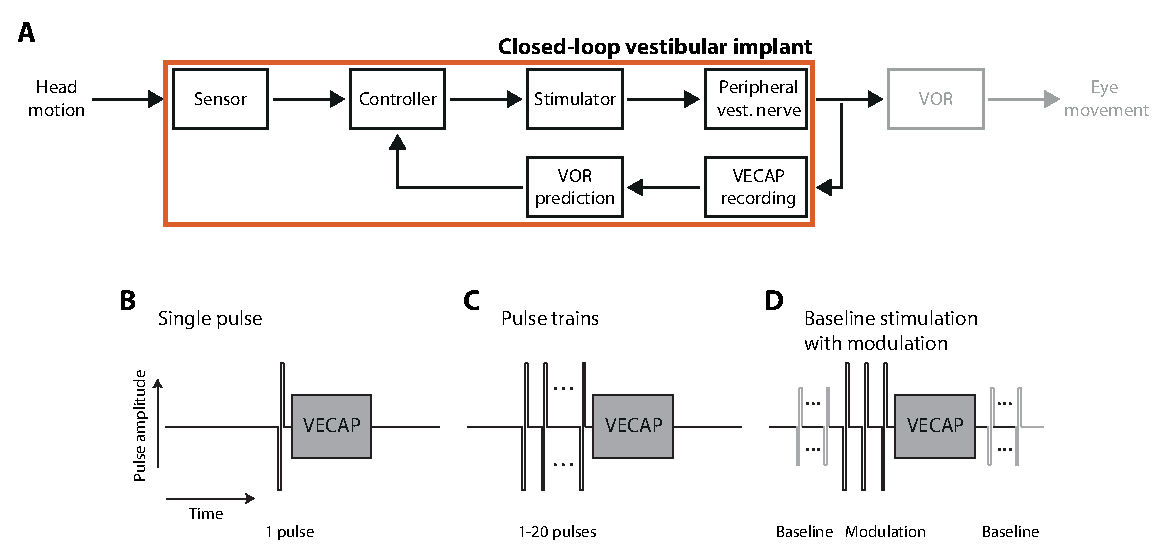
\includegraphics[width=\textwidth]{chapters/partI/vecapvor/figures/Fig_vecapvor_closedloop.eps} 
\caption[Closed-loop VI concept for a vestibular implant and VECAP test paradigm]{Closed-loop VI concept for a vestibular implant and VECAP test paradigm. (\textbf{A}) An expansion of the scheme in Fig.\,\ref{fig:viconcept} with a closed-loop. For gaze stabilization, head motion would entail a countering and compensating VOR response, a VOR reference trajectory. VECAP recording could be utilized to predict VOR response and adjust stimulation settings to reduce error. (\textbf{B}-\textbf{D}) VECAP and VOR were recorded to single pulses, pulse trains (1, 2, 5, 10 and 20 pulses) and with baseline stimulation.}
\label{fig:vecapvor:closedloop}
\end{figure}

\subsection{Specific stimulation and recording paradigms}
Figure\,\ref{fig:vecapvor:closedloop}B-D illustrate the three experiments. VOR and VECAP were both measured for all experiments. 

\subparagraph{Single pulses} VECAP and VOR responses were recorded to at least seven different pulse amplitudes linearly spaced between \SI{0}{\micro\ampere} and the maximum current level limited by the compliance voltage of the stimulator (Fig.\,\ref{fig:vecapvor:closedloop}B). VECAP and VOR were separately recorded since the electromagnetic field for VOR recording would have affected the VECAP recording. Maximum levels, stimulation and recording electrodes for each subject are listed in Table\,\ref{tab:vecapvor}.
   
\subparagraph{Pulse trains}
Prior to the application of the pulse trains, the subject was not adapted to any baseline stimulation. First, VOR was recorded to pulse trains of 1, 2, 5, 10 or 20 pulses at a pulse rate of 250 pulses per second (pps). These trains consisted only of probe pulses with a constant pulse amplitude at 60\% of the maximum level. Afterwards the coil system was turned off for VECAP recording.

VECAP was recorded to the same pulse trains. The set of pulse trains was repeated three times to record responses to probe, masker-probe and masker pulses (Fig.\,\ref{fig:vecapvor:closedloop}C).

\subparagraph{VECAP during baseline stimulation}  
Subject 3 was freely moving in a small cage, in contrast to the other head-restrained experiments. VOR was not recorded and the search coil system was off. Baseline stimulation was turned on for four 30-minute periods. Pulse rate was 250\,pps, current amplitude 160\,cu. Other pulse settings were unchanged. VECAP was recorded in intervals of three minutes with the full masker-probe paradigm. A complete recording cycle of 30 iterations for probe, masker-probe and masker took 765 ms, i.\,e. no baseline stimulation was applied during that period. 

\subparagraph{VECAP to pulse amplitude steps after adaptation to baseline stimulation}
This experiment shared some similarities with the study reported in Chap.\,\ref{chap:pamprm}. Subjects 3 and 4 were subjected to baseline stimulation for 12 minutes (Saginaw et al., 2010) with the baseline pulse amplitude at 50\% of the maximal level. Afterwards five pulses at a different pulse amplitude (lower or higher than baseline pulse amplitude) were applied and the responses recorded. VECAP and VOR were again recorded separately (Fig.\,\ref{fig:vecapvor:closedloop}D). 

{\footnotesize
\hyphenation{elec-trode}
\begin{table}
\begin{threeparttable}[tbp]\footnotesize
\caption{Stimulation and recording settings for VECAP-VOR study}\label{tab:vecapvor}
\begin{tabularx}{\textwidth}{>{\centering\arraybackslash}m{.13\textwidth}>{\centering\arraybackslash}m{.18\textwidth} >{\centering\arraybackslash}m{.18\textwidth} >{\centering\arraybackslash}m{.18\textwidth} >{\centering\arraybackslash}m{.23\textwidth}}
\toprule
Subject & Lower threshold [cu] & Maximum level [cu] & Stimulation electrode site & Recording electrode sites \\
\midrule
Sub1 & 420 & 720 & 4 & 8-5\\
Sub2 & 200 & 600 & 2 & 1-3\\
Sub3 & 190 & 315 & 2 & 4-7\\
Sub4 & 200 & 450 & 7 & 1-6\\
\bottomrule
\end{tabularx}
\begin{tablenotes}
\item Stimulation was monopolar in all cases, the return electrode was an electrode in the neck musculature.
\item The second electrode for served as recording ground.
\end{tablenotes}
\end{threeparttable}
\end{table}
}
\section{Results}
\subsection{VECAP-VOR Correlation to Single Pulses}
VOR responses were measured to the probe pulse with  different amplitudes ranging from 0 to the maximum pulse amplitude. Figure\,\ref{fig:vecapvor:single}A illustrates an example of  VECAP after processing with the masker-probe technique. Figure\,\ref{fig:vecapvor:single}B shows an example of averaged horizontal VOR velocity to \SI{600}{\micro\ampere} stimulation in subject 1 (Sub1). Stimulation of the horizontal canal evoked predominantly horizontal VOR response with only small, negligible vertical VOR (ratio ca. 4:1, we therefore focused on horizontal VOR responses for the remainder of this chapter). Velocities peaked at about 7 ms after stimulation onset, which is typical for this species.

Figure\,\ref{fig:vecapvor:single}C relates normalized PEV to pulse amplitude for all four subjects. They all revealed a piecewise linear pattern with a marked increase in PEV beyond a certain N-P voltage. Up to that inflection point, N-P voltage increased, while no or little VOR response was evoked. The inflection points were different for all subjects: 0.78, 0.87, 0.66 and  0.5 for Sub1 through Sub4.  respectively. Piecewise linear fits to the data were good with r$^2$\,\textgreater\,0.75, and best for Sub4 with 0.969. 
\begin{figure}[btp]
\centering
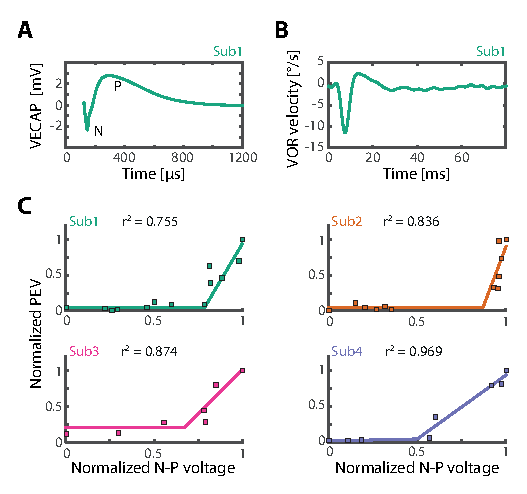
\includegraphics{chapters/partI/vecapvor/figures/Fig_vecapvor_single.eps} 
\caption[VECAP-VOR correlation to single pulses]{VECAP-VOR correlation to single pulses. (\textbf{A}) VECAP recording in Sub1 at 600\,$\mu$A had clear N and P waves. (\textbf{B}) The horizontal VOR velocity to the same single pulse as in (A). The negative velocity indicated eye movement to the right. (\textbf{C}) VECAP-VOR correlation to single pulses for all four subjects. The piecewise linear pattern was evident in all subjects. However, they had different inflection points and  slopes.}
\label{fig:vecapvor:single}
\end{figure}

\subsection{VECAP-VOR Correlation to Pulse Trains}
The time course of eye velocity for Sub3 and for different pulse numbers are shown in Fig.\,\ref{fig:vecapvor:trains}A. PEVs occurred approx. \SI{8}{\milli\second} after the end of the pulse train for 1 and 2 pulses (10 and \SI{12.5}{ms}, respectively). For the other cases, velocity peaked before the end of the train (e.\,g., at 15 ms for 10 pulses). After the peak, velocity returned to zero with a small negative overshoot for 1 and 2 pulses. For 5 pulses, velocity decreased rapidly with the end of the train. For 10 and 20 pulses, velocity declined slowly first and then rapidly with the end of the train (inflection points at 40.8 and \SI{81.8}{\micro\second}, respectively).

PEV increased with pulse number up to 5 pulses with a gain less than unity (normalized PEV in Fig.\,\ref{fig:vecapvor:trains}B). Specifically, PEV for 5 pulses was 3.6 times larger than PEV for 1 pulse. For 10 and 20 pulses, PEV did not increase further and was similar to PEV for 5 pulses.  

Normalized N-P voltage of VECAP is shown in Fig.\,\ref{fig:vecapvor:trains}C. N-P voltage was highest after 1 pulse. It then trended down up to 5 pulses and remained relatively unchanged for more pulses. The differences in N-P voltage were not significant (2-sample Kolmogorov-Smirnov test, p\,\textgreater\,0.47 for Sub3).
Latencies for the negative wave were constant at \SI{150}{\micro\second} after stimulation onset. Also the latencies for the positive wave remained stable at ca. \SI{250}{\micro\second} (not shown).
 
\begin{figure}[btp]
\centering
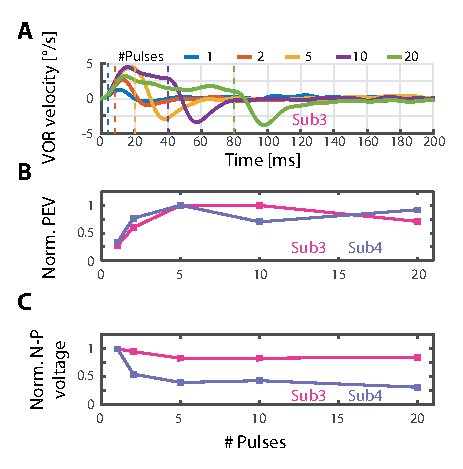
\includegraphics{chapters/partI/vecapvor/figures/Fig_vecapvor_trains2.eps} 
\caption[VECAP-VOR correlation to pulse trains]{VECAP-VOR correlation to pulse trains. (\textbf{A}) VOR velocity in Sub3 for different pulse trains with 1 to 20 pulses. The vertical dashed lines mark the end of the corresponding pulse train. (\textbf{B}) Normalized PEV for Sub3 and Sub4. Both had the same trend; an increase of PEV until five pulses and then a plateau. (\textbf{C}) Normalized N-P voltage in the same subjects. The highest value occurred after a single pulse and declined insignificantly until five pules.
}
\label{fig:vecapvor:trains}
\end{figure}

\subsection{VECAP-VOR Correlation with Baseline Stimulation}
In Fig.\,\ref{fig:vecapvor:baseline}A, the N-P voltage showed an increasing trend with time, but the differences were insignificant (2-sample KS-test, p\,\textgreater\,0.05). Latencies for N and P waves did not change significantly over 30-minutes. P wave latency oscillated between 220 and \SI{240}{\micro\second}, while N wave latency was constant at \SI{122.5}{\micro\second}. 

After adaptation to acute continuous stimulation, subjects were head restrained to measure both VECAP and VOR. While continuing baseline stimulation, brief pulse trains of different pulse amplitude were applied. Specifcally, five pulses were applied with lower or higher pulse amplitude than baseline pulse amplitude. These steps elicited bidirectional VOR responses in Sub3, i.\,e., left or right. In Sub4, higher pulse amplitude evoked a clear directional VOR response, while lower pulse amplitude had no effect. Figure\,\ref{fig:vecapvor:baseline}C shows the correlation between VECAP and PEV. The linear fit was good for Sub3, although only four pulse amplitude steps were tested (r$^2$ = 0.987). For Sub4, r$^2$ was 0.471 due to the weak VOR response for lower pulse amplitudes.

The recording time of \SI{765}{\milli\second} every three minutes should have had no major impact on the nerve state (the recording delivered 90 pulses in the same period that 191 baseline pulses would be expected). Total recording time constituted \SI{8.4}{s} or less than 0.5\% of stimulation time. 

\begin{figure}[btp]
\centering
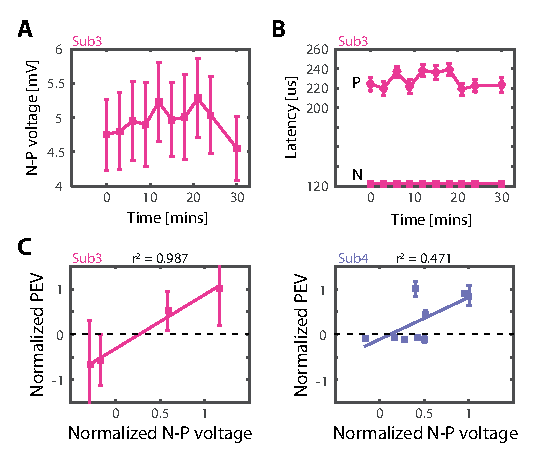
\includegraphics{chapters/partI/vecapvor/figures/Fig_vecapvor_baseline2.eps} 
\caption[VECAP-VOR correlation with baseline stimulation]{VECAP-VOR correlation with baseline stimulation. (\textbf{A})-(\textbf{B}) VECAP recording in Sub3 at baseline stimulation every 3 minutes over 30 minutes. Neither N-P voltage nor N or P latencies did change significantly in magnitude . (\textbf{C}) After continuous baseline stimulation, brief pulse trains of 5 pulses with lower or higher pulse amplitude were applied to evoke bidirectional responses and record according VECAP. Sub3 showed bidirectional VOR responses and a linear function was fitted to the data. Sub4 showed only VOR responses to pulse trains with higher than baseline pulse amplitude and a fit had low r$^2$ value. (Error bars in Sub4 were smaller than the marker.)}
\label{fig:vecapvor:baseline}
\end{figure}

\section{Discussion}
\subsection{VECAP-VOR Correlation}
We studied the correlation between VECAP and VOR response to single pulses, pulse trains and with baseline stimulation. VECAPs in the literature have been proposed as intraoperative tool for electrode placement and was successful in animal instrumentation (Nie et al., 2011). One group also presented an abstract at the meeting of the Association of Research in Otolaryngology (Dai et al., 2012b), reporting VECAP and VOR responses to single pulses in a rhesus monkey, similar to the ones presented herein.

\subparagraph{Single pulses} The single pulse responses were the first step towards VOR prediction with VECAP and showed a piecewise linear pattern. For below threshold pulse amplitudes, N-P voltage increased, while no VOR response was evoked. For above threshold pulse amplitudes, PEV increased together with N-P voltage. The pattern was expected: We anticipated VECAP to gauge vestibular nerve activation before any visible VOR response. However, it is not certain what the exact mechanism is. One hypothesis is that VOR onset requires a minimum amount of nerve activity or a minimum number of action potentials which would represent a detection threshold. A second hypothesis is that below threshold stimulation preferentially recruits irregular afferents because of their higher sensitivity to galvanic electrical stimulation. Stronger pulse amplitudes then recruit regular afferents that play a more important role in the VOR response than irregular afferents (Minor and Goldberg, 1991). If the second hypothesis were true, and if one could specifically stimulate regular afferents, then this could lead to a more efficient vestibular implant. A combination of VECAP, single unit and VOR recording could address this question.

Clinically more relevant, the inflection points of the piecewise liner fits could be used for subject-specific automatic threshold estimation. The points of the fits and the slopes of the rising part of the pattern were different for each subject. This was due to the different dynamic ranges, i.\,e. the difference between lower, vestibular threshold and maximal level (Table\,\ref{tab:vecapvor}). A small range would result in an inflection at high normalized N-P voltage and higher slope, such as with Sub2 (Fig.\,\ref{fig:vecapvor:single}C). These dynamic ranges are difficult to control for and depend on precise electrode placement, the individual tissue-electrode reaction and, in patients, also on etiology and status of the nerve. (In our animal model, vestibular pathology was induced by electrode insertion into the ampulla and rendering the canals insensitive to rotation.) Ideally one would strive for a maximum possible dynamic range to have more available pulse amplitudes.   

\subparagraph{Pulse trains}
Pulse trains generated larger VOR responses than single pulses. This is relevant since VOR responses to single pulses are likely to be insufficient for daily activity (e.\,g., for Sub1 PEV -11.5\,\degree /s or 0.05\degree eye movement). However, our findings revealed that PEV only increased for pulse trains up to five pulses. 

More tests will be required to explain the phenomenon. Tests herein were performed at a pulse rate of 250\,pps and higher pulse rates may evoke higher PEV. In fact, in a singular test we applied 3000\,pps in Sub3 (D. Jiang, \textit{pers. comm.}, February 2013). We evoked higher PEV and the maximum was obtained with 20 pulses. One possible explanation might be eye muscle fatigue. Muscle fibers are able to exert maximum force (i.\,e., maximum acceleration) in response to the first pulse(s), but are not able to sustain that force level afterwards because of the preceding muscle twitch and insufficient recovery time. For instance, twitch time in monkeys was measured between 6 and \SI{8}{\milli\second} (Fuchs and Luschei, 1971) and would fit the observation that PEV for 5, 10 and 20 pulses at 250\,pps occurred around \SI{10}{\milli\second}.

N-P voltage was stable and did not change significantly for different pulse trains. Although differences were insignificant, the downward trend from 1 to 5 pulses could be viewed as a transition from an impulse response to a steady state. The stable latencies for N and P waves further indicate that neither the shape of VECAP changed with pulse number. This was no surprise. From the previous chapter, we learnt that VECAP to a single pulses recovered within \SI{1}{\milli\second}. Similarly, VECAPs in rhesus monkey returned to baseline within that time (Nie et al., 2011). Here, the pulses were applied every 4 ms, which gave sufficient recovery time.

\subparagraph{Baseline stimulation}
VECAP was recorded in three minute intervals during 30 minutes of continuous stimulation. No significant change in N-P voltage was observed as expected. VECAP recovers to baseline within \SI{1}{\milli\second}, therefore continuous stimulation at 250\,pps (a pulse every \SI{4}{\milli\second}) should not affect VECAP \emph{at this time scale}. Long-term continuous stimulation over one week or longer could initiate changes at the electrode-tissue interface that in turn could alter electrode impedance and VECAP (Phillips et al., 2014).

Applying pulse amplitude steps lower or higher than baseline pulse amplitude successfully evoked bidirectional VOR responses in Sub3. In Sub4, only higher than baseline pulse amplitudes evoked a unidirectional. A linear function was fitted to the data and could be used to estimate VOR from VECAP. Though the fit had a high r$^2$ value for Sub3, VOR variance was large (on average 38.3\% of mean). In Sub4, variance was low, but r$^2$ was less than 0.5. We had hoped to see a linear relation between N-P voltage and PEV, but did not expect standard deviation as large as observed. The results in Sub4 might be related to a device problem in the cochlear implant that we noticed shortly after and could explain why lower than baseline pulse amplitudes did not evoke a VOR response. 

\subsection{Closed-loop Control for Vestibular Implant}
In the proposed closed-loop VI, the N-P voltage from VECAP recordings would be utilized to predict the VOR response output and to adjust stimulation parameters to reduce output error. VECAP has the advantage of a shorter latency (\SI{1}{\milli\second}) than the optokinetic system that only uses visual feedback (5-\SI{10}{\milli\second}). 

Our findings can be regarded as first stepping stone and are promising in that regard. However, to achieve a closed-loop VI requires more research and testing. First, we have related N-P voltage only to PEV, a parameter that does not contain information about the time course of the VOR response. To follow a reference VOR trajectory, a controller could view that trajectory as sequence of PEVs.

Second, PEV is also dependent on the number of applied pulses. Since VECAP did not change significantly with the number of pulses, the number and likely also eye muscle fatigue would have to be taken into account for PEV. This parameter is known to the controller. 

Third, the prediction is dependent on the baseline stimulation. It facilitated bidirectional VOR responses. The computed linear fit may shift with baseline pulse amplitude and would have to be learned specifically for the applied baseline pulse amplitude.

Fourth, the prediction with VECAP is currently only compatible with pulse amplitude modulation. Pulse rate modulation would yield different and lower VOR responses (cf.\,Chap.\,\ref{chap:pamprm}), but would not change VECAP output that is driven by pulse amplitude. One approach would be to additionally include the pulse rate in the prediction, also a parameter known to the controller.

Finally, the variance in both VECAP and VOR was substantial. The variance in VECAP is related to an offset in the recording unit of the cochlear implant. It could be reduced with better internal settings  we had no access to. The variance in VOR is likely related to the small PEVs evoked (ca. 5\,\degree /s) and thus small signal-to-noise ratio. More typically required PEV would be around 30\,\degree /s (Merfeld et al., 2007; Perez-Fornos et al., 2014). To achieve these PEVs, higher stimulation rates greater than 500\,pps are necessary as longer phase width would impede VECAP recording. However, high pulse rates may entail other effects such as desynchronization of afferents that have not been studied in the vestibular system, but to some extent in the cochlear system (Litvak et al., 2003).

\section{Summary}
VECAP and VOR responses were recorded to single pulses, pulse trains and with baseline stimulation. Responses from single pulses could be clinically used for automatic threshold estimation which would be more time efficient than the current practice of applying stimulation - inquiring patient - increasing stimulation - inquiring patient etc.  Though we found correlations between the responses, they would not be sufficiently robust for a closed-loop VI for the time being. Responses to pulse trains and with baseline stimulation were encouraging, but also revealed that a closed-loop VI will require  more research and testing.